\documentclass[a4paper, 11pt]{article}

\usepackage[absolute]{textpos} % absolute positioned text blocks
\setlength{\TPHorizModule}{1mm}
\setlength{\TPVertModule}{1mm}
\usepackage[english]{babel}
\usepackage{csquotes}

% Images
\usepackage{graphicx,wrapfig} % used for images
\graphicspath{ {./img/} }
\usepackage[labelfont=bf]{caption}

% Formatting
\usepackage{geometry} % better margins for document
\usepackage{titlesec} % better control over title spacing 
\usepackage{tabularx} % better tables
\usepackage[hidelinks]{hyperref} % hrefs
\usepackage{totcount}
\usepackage{pgfplots}
\pgfplotsset{compat=1.16}
\pgfplotsset{
    colormap={cool}{rgb255(0cm)=(237,66,76); rgb255(0.5cm)=(255,255,255); rgb255(1cm)=(57,146,239)}
}
\usepgfplotslibrary{colorbrewer}

\usepackage{float} % image placement
\usepackage{amssymb} % math symbols

% Code listings
\usepackage{listings}
\usepackage{commath}
\usepackage{pifont}
\usepackage[misc,weather,alpine]{ifsym}
\usepackage{xcolor}
\definecolor{codered}{rgb}{0.93,0.26,0.298}
\definecolor{codegrey}{rgb}{0.7,0.7,0.7}
\definecolor{codepink}{rgb}{0.737,0.47,0.823}
\definecolor{codeblue}{rgb}{0.227,0.572,0.937}
\definecolor{codegreen}{rgb}{0.441,0.664,0.286}
\definecolor{codestring}{rgb}{0.58,0,0.82}
\definecolor{backcolor}{rgb}{0.95,0.95,0.95}
\definecolor{lightgrey}{rgb}{0.8,0.8,0.8}
\definecolor{darkcyan}{RGB}{0,115,192}

\lstdefinelanguage{HLSL}{
	morekeywords=[1]{
        % variables
        position,sphere,direction,stepSize,dirMultiplier,dScene,dOrigin,p,dMin,dMax,result,k,d1,d2,d3,i,ao,co,d,seed,cell,pCell,
        i,j,x,y,z,frequency,amplitude,current,total,maxValue,
        vpos,ppos,vd,pd,density,projectedSunDistance,sunColor,sunTransmittance,cloudDensity,worldPosition,
        lightTransmittance,sunDirection,lightStepSize,insideBoxDist,
	},
	morekeywords=[2]{
        % methods and functions
		distance,normalize,min,max,dot,pow,sin,cos,tan,fract,length,smoothstep,
        sphereHit,raymarch,sphereDistance,sceneSDF,estimateNormal,hardshadow,softshadow,blend,sphereSDF,boxSDF,
        difference,union,intersection,ambientOcclusion,voronoi,
        random2d,random,random3d,randomSeed,floor,fbm,
        noise,lightmarch,
        sampleDensity,getColorVoronoi,getColorPerlin,worldToScreenPos
	},
	morekeywords=[3]{
        % CONSTANTS
        STEP_SIZE,MAX_STEPS,MINIMUM_STEP_SIZE,SURFACE_DISTANCE,MAX_DISTANCE,EPSILON,
        AO_ITERATIONS,AO_INTENSITY,AO_STEP_SIZE,
        LACUNARITY,GAIN,OCTAVES,
    },
	% morekeywords=[4]{
    %     % Unity Variables
    %     _VoronoiScale,_VoronoiOffset,,_VoronoiOctaves,_VoronoiPersistance,_VoronoiDensityThreshold,_VoronoiDensityMultiplier,
    %     _PerlinScale,_PerlinOffset,_PerlinOctaves,_PerlinPersistance,_PerlinDensityThreshold,_PerlinDensityMultiplier,
    % },
    keywordstyle=[1]\color{codeblue},
    keywordstyle=[2]\color{codered},
    keywordstyle=[3]\color{codepink},
    % keywordstyle=[4]\color{codegreen},
	commentstyle=\color{codegrey},
	morestring=[b]", % defines that strings are enclosed in double quotes
	morestring=[b]', % defines that strings are enclosed in single quotes
    backgroundcolor=\color{backcolor},
    stringstyle=\color{codered},
    numberstyle=\tiny,
    basicstyle=\ttfamily\footnotesize,
    breakatwhitespace=false,
    breaklines=true,
    captionpos=b,
    keepspaces=true,
    numbers=left,
    numbersep=5pt,
    showspaces=false,
    showstringspaces=false,
    showtabs=false,
	tabsize=2,
    sensitive=false, % keywords are not case-sensitive
    morecomment=[l]{//}, % l is for line comment
    morecomment=[s]{/*}{*/}, % s is for start and end delimiter
    belowskip=2.5em,
    aboveskip=1em,
}

% Gantt charts
\usepackage{pgfgantt}

% drawings
\usepackage{tikz}
\usepackage{fontawesome}
\usetikzlibrary{positioning, shapes}
\usetikzlibrary{arrows.meta}
\geometry{
	a4paper,
	left=28mm,
	right=28mm,
    top=30mm,
    bottom=30mm
}

% Colors 
\RequirePackage{color}
\definecolor{bfhgrey}{rgb}{0.41,0.49,0.57}
\definecolor{brinkpink}{rgb}{1.0, 0.65, 0.79}
\definecolor{columbiablue}{rgb}{0.61, 0.87, 1.0}

% Glossary
\usepackage[toc]{glossaries}
% Acronyms
\newglossaryentry{hlsl}{name={HLSL}, text={HLSL}, first={high-level shading language (HLSL)}, description={High-level shading language. Developed by microsoft, this is a standard shader language for DirectX used in graphics programming}}
\newglossaryentry{json}{name={JSON}, text={JSON}, first={Java-Script object notation (JSON)}, description={Java-Script object notation. A light-weight data format that is stored as human-readable text}}
\newglossaryentry{slpk}{name={SLPK}, text={SLPK}, first={ESRI scene layer package (SLPK)}, description={ESRI scene layer package A custom, web-optimized format used for files related to ESRI }}
\newglossaryentry{png}{name={PNG}, text={PNG}, first={portable network graphic (PNG)}, description={Portable network graphic. A common format for lossless compressed image files}}
\newglossaryentry{ui}{name={UI}, text={UI}, first={user interface (UI)}, description={User interface. The interface that allows the user to interact with the software}}
\newglossaryentry{gpu}{name={GPU}, text={GPU}, first={GPU}, description={Graphics processing unit. A piece of hardware designed to rapidly manipulate and alter memory, often intented for output to a display device}}
\newglossaryentry{wmo}{name={WMO}, text={WMO}, first={World Meteorological Organization (WMO)}, description={A specialized agency conducting atmospheric science, climatology, hydrology and geophysics}}

% Glossary entries
\newglossaryentry{latex}{name=LaTeX, description={ A high-quality document preparation system designed for the production of technical and scientific documentation }}
\newglossaryentry{noisegeneration}{name=Noise generation, text={noise generation}, description={ Noise generation is used to generate textures of one or more dimension with seemingly random smooth transitions from black to white (zero to one) }}
\newglossaryentry{volumetric}{name=Volumetric, text={volumetric}, description={ This describes a technique which takes a 3D volume of data and projects it to 2D. It is mostly used for transparent effects stored as a 3D image }}
\newglossaryentry{raymarching}{name=Ray marching, text={ray marching}, description={ Ray marching is a type of method to approximate the surface distance of a volumetric object, where a ray is cast into the volume and stepped forward until the surface is reached }}
\newglossaryentry{lightmarching}{name=Lightmarching, text={lightmarching}, description={ The same concept as \gls{raymarching}, but instead of being cast into the volume, it is cast towards the primary light source with a constant step }}
\newglossaryentry{billboard}{name=Billboard, text={billboard}, description={ A 2D image always facing towards the main camera }}
\newglossaryentry{worldspace}{name=World space, text={world space}, description={ Coordinates defined with respect to a global Cartesian coordinate system }}
\newglossaryentry{polymesh}{name=Polymesh, text={polymesh}, description={ A polymesh is a 3D model composed of polygons or triangles }}
\newglossaryentry{lowpoly}{name=Low poly, text={low poly}, description={ A 3D polymesh with a relatively low count of polygons }}
\newglossaryentry{voxel}{name=Voxel, text={voxel}, description= { Short for \textit{volume element}, a voxel is a value (either a number or a vector) on a scalar or vector field }}
\newglossaryentry{scalarfield}{name=Scalar field, text={scalar field}, description={ A scalar field describes a typically three-dimensional grid of elements called \textit{voxels}, each containing a scalar value }}
\newglossaryentry{vectorfield}{name=Vector field, text={vector field}, description={ It is the same as a scalar field, except the voxels are vector values }}
\newglossaryentry{spheretracing}{name=Sphere tracing, text={sphere tracing}, description={ Sphere tracing describes an optimized algorithm of ray marching by using signed distance functions to approximate the surface distance of the volume }}
\newglossaryentry{sdf}{name=Signed distance function, text={signed distance function}, description={ A signed distance function, short SDF, returns a positive distance if the origin is outside the volume and a negative distance if it is inside the volume }}
\newglossaryentry{surfacenormal}{name=Surface normal, text={surface normal}, description={ A \textit{surface normal} or \textit{normal} is a vector which is perpendicular to a given geometry, like a triangle or polygon }}
\newglossaryentry{gradient}{name=Gradient, text={gradient}, description={ The \textit{gradient} denotes the direction of the greatest change of a scalar function }}
\newglossaryentry{penumbra}{name=Penumbra, text={penumbra}, description={ The partially shaded outer region of diffuse shadows. Also described as soft edges }}
\newglossaryentry{shapeblending}{name=Shape blending, text={shape blending}, description={ In SDFs, shapes can be seemingly blended together by returning a interpolated value of those distances }}
\newglossaryentry{ambientocclusion}{name=Ambient occlusion, text={ambient occlusion}, description={ Also known as contact shadows, this method darkens points in the scene that are not or only slightly exposed to the light and its environment }}
\newglossaryentry{noise}{name=Noise, text={noise}, description={ A randomly generated pattern, referring to \gls{procedural} pattern generation }}
\newglossaryentry{translucent}{name=Translucent, text={translucent}, description={ An object or substance that is translucent allows light to be passed through it, meaning it is rendered transparently to some degree }} 
\newglossaryentry{parameters}{name=Parameters, text={parameters}, description={ Shader variables exposed to the Unity Editor }} 
\newglossaryentry{sss}{name=Subsurface scattering, text={subsurface scattering}, description={ SSS is a mechanism of light transport in which light enters a translucent object, is scattered around and exits the material at a different point, resulting in illuminated areas where the material is thin }} 
\newglossaryentry{sunlightforwarding}{name=Sunlight forward scattering, text={sunlight forward scattering}, description={ The process of sunlight shining through and illuminating the clouds which cover the sun }} 
\newglossaryentry{sunlighttransmittance}{name=Sunlight transmittance, text={sunlight transmittance}, description={ In this matter, the same as \gls{sunlightforwarding} }} 
\newglossaryentry{cnn}{name=Convolutional neural network, text={convolutional neural network}, description={ A neural network that is able to classify images }} 
\newglossaryentry{gan}{name=Generative adverserial network, text={generative adverserial network}, description={ A set of two neural networks, where one generates images and the other tries to tell wether those images are real or generated }} 
\newglossaryentry{aabb}{name=Axis-aligned bounding box, text={axis-aligned bounding box}, description={ A non-rotated bounding box enclosing an object completely }} 
\newglossaryentry{shader}{name=Shader, text={shader}, description={ A piece of software which runs on the \gls{gpu}, rendering geometrically defined objects to the screen  }} 
\newglossaryentry{computeshader}{name=Compute shader, text={compute shader}, description={ A shader which runs on the GPU but outside of the default render pipeline }} 
\newglossaryentry{fbm}{name=Fractal Brownian motion, text={fractal Brownian motion}, description={ Different iterations of continuously more detailed noise layered on top of each other }} 
\newglossaryentry{fractalnoise}{name=Fractal noise, text={fractal noise}, description={ In this matter, the same as \gls{fbm} }} 
\newglossaryentry{procedural}{name=Procedural, text={procedural}, description={ Created solely with algorithms and independant of any prerequisites }}
\newglossaryentry{histogram}{name=Histogram, text={histogram}, description={ A graphical representation of data like brightness or color distribution of a given photograph }}
\newglossaryentry{csg}{name=Constructive solid geometry, text={constructive solid geometry}, description={ Short CSG, stands for combining primitive geometric objects with Boolean operators }}
\newglossaryentry{neuralnetwork}{name=Neural network, text={neural network}, description={ A series of algorithms that can recognize and categorize certain patterns in a given set of data }}
\newglossaryentry{interpolation}{name=Interpolation, text={interpolation}, description={ In mathematics, interpolation describes a method of estimating unknown values that fall between known values }}
\newglossaryentry{wrs}{name=Weather rendering system, text={weather rendering system}, description={ The Unity application that is implemented during this project. It takes in live data from a weather service and uses topological elevation models to create a weather simulation, which is then rendered and up for comparison with live photographs }}
\newglossaryentry{altitude}{name=Altitude, text={altitude}, description={ A vertical distance measurement, in this context specifically the distance from sea level to the given object }}
\newglossaryentry{watervapor}{name=Water vapor, text={water vapor}, description={ Evaporated water in a gaseous form }}
\newglossaryentry{desublimation}{name=Desublimation, text={desublimation}, description={ The process of gas transitioning to liquid without passing through the liquid phase }}
\newglossaryentry{halophenomenon}{name=Halo phenomenon, text={halo phenomenon}, description={ White or colored rings or arcs of light around the sun or the moon, produced by cirrostratus clouds }}
\newglossaryentry{cloudlet}{name=Cloudlet, text={cloudlet}, description={ Small, white, puffy clouds that come in large quantities, together forming a cloud of the cumulus family }}
\newglossaryentry{precipitation}{name=Precipitation, text={precipitation}, description={ Rainfall. The result of atmospheric water vapor that has been condensed and now falls from clouds }}
\newglossaryentry{convection}{name=Convection, text={convection}, description={ The process of warm air rising from the surface and cooling at higher altitude, of which the moisture is then condensed into clouds }}
\newglossaryentry{thermal}{name=Thermal, text={thermal}, description={ In relation with meteorology, the hot, rising air from convection is called "thermal" }}
\newglossaryentry{weatherfront}{name=Weather front, text={weather front}, description={ A boundary between to air masses, which differ in temperature, wind direction and humidity }}
\newglossaryentry{warmfront}{name=Warm front, text={warm front}, description={ A warm \gls{weatherfront}, the boundary of a mass of air that carries mild or warm air. When colliding with a \gls{coldfront}, \gls{precipitation} is often followed }}
\newglossaryentry{coldfront}{name=Cold front, text={cold front}, description={ A cold \gls{weatherfront}, the boundary of a mass of air that carries cold or cool air. When colliding with a \gls{warmfront}, \gls{precipitation} is often followed }}
\newglossaryentry{occludedfront}{name=Occluded front, text={occluded front}, description={ When a cold front overtakes a warm front, it pushes the warm air upwards (\gls{thermal}s). The moisture of the warm air condenses as it rises, creating \gls{watervapor}. This often results in clouds with \gls{precipitation} }}
\newglossaryentry{occlusion}{name=Occlusion, text={occlusion}, description={ In meteorology, the clash of a warm front and a cold front. See \gls{occludedfront} }}
\newglossaryentry{lerp}{name=Linear interpolation, text={linear interpolation}, description={ Simply put, linear interpolation describes a method of finding values inbetween two points on the same line }}
\newglossaryentry{particlesystem}{name=Particle system, text={particle system}, description={ In computer graphics, a particle system is a technique that continuously spawns and recycles objects. They are often used to reproduce fire or smoke effects, with small flame or dust textures as particles }}
\newglossaryentry{pseudorandom}{name=Pseudo-random, text={pseudo-random}, description={ A random number generated with a deterministic algorithm, meaning that the same input will always give the same output }}
\newglossaryentry{textureslice}{name=Texture slice, text={texture slice}, description={ A 2D texture extracted from a 3D texture for a given depth }}

\makenoidxglossaries

\glsunset{gpu}

% Bibliography
\usepackage[backend=biber, style=ieee]{biblatex}
\addbibresource{partials/paper.bib}

% add another lavel of headings
%\setcounter{tocdepth}{4}
\setcounter{secnumdepth}{4}
\titleformat{\paragraph}
{\normalfont\normalsize\bfseries}{\theparagraph}{1em}{}
\titlespacing*{\paragraph}
{0pt}{3.25ex plus 1ex minus .2ex}{1.5ex plus .2ex}

\begin{document}

\color{black}

\title{\doctitle}
\author{\docauthor}
\date{\versiondate}

\newcounter{requirements}
\newtotcounter{versionnumber}
\newcommand{\docsubtitle}{Project documentation}
\newcommand{\docauthor}{Matthias Thomann}
\newcommand{\doctitle}{Real-time Weather Rendering System}
\newcommand{\fieldofstudies}{BSc in Computer Science}
\newcommand{\specialisation}{Computer perception and virtual reality}
\newcommand{\prof}{Prof. Urs K\"unzler}

\newcommand{\versiondate}{\today}
\newcommand{\sectionref}[1]{\autoref{#1}}
\newcommand{\emptyline}{\vspace{\baselineskip}\\\noindent}

\titlespacing*{\section} {0pt}{7.5ex plus 1ex minus .2ex}{2.3ex plus .2ex}
\titlespacing*{\subsection} {0pt}{4.25ex plus 1ex minus .2ex}{1.5ex plus .2ex}

\pagenumbering{roman}
\setcounter{page}{3}

%% include BFH logo and HuCE-ml logo

\begin{titlepage}

\setlength{\unitlength}{1mm}

\begin{textblock}{20}[0,0](22,12)
    
\includegraphics{../img/BFH_Logo_B.png}
\end{textblock}

\begin{flushleft}

\vspace*{21mm}

\fontsize{24.88pt}{40pt}\selectfont
\textbf{\doctitle}
\vspace{2mm} 

\fontsize{17.28pt}{24pt}\selectfont\vspace{0.3em}
\docsubtitle
\vspace{6mm}

\begin{figure}[H]
    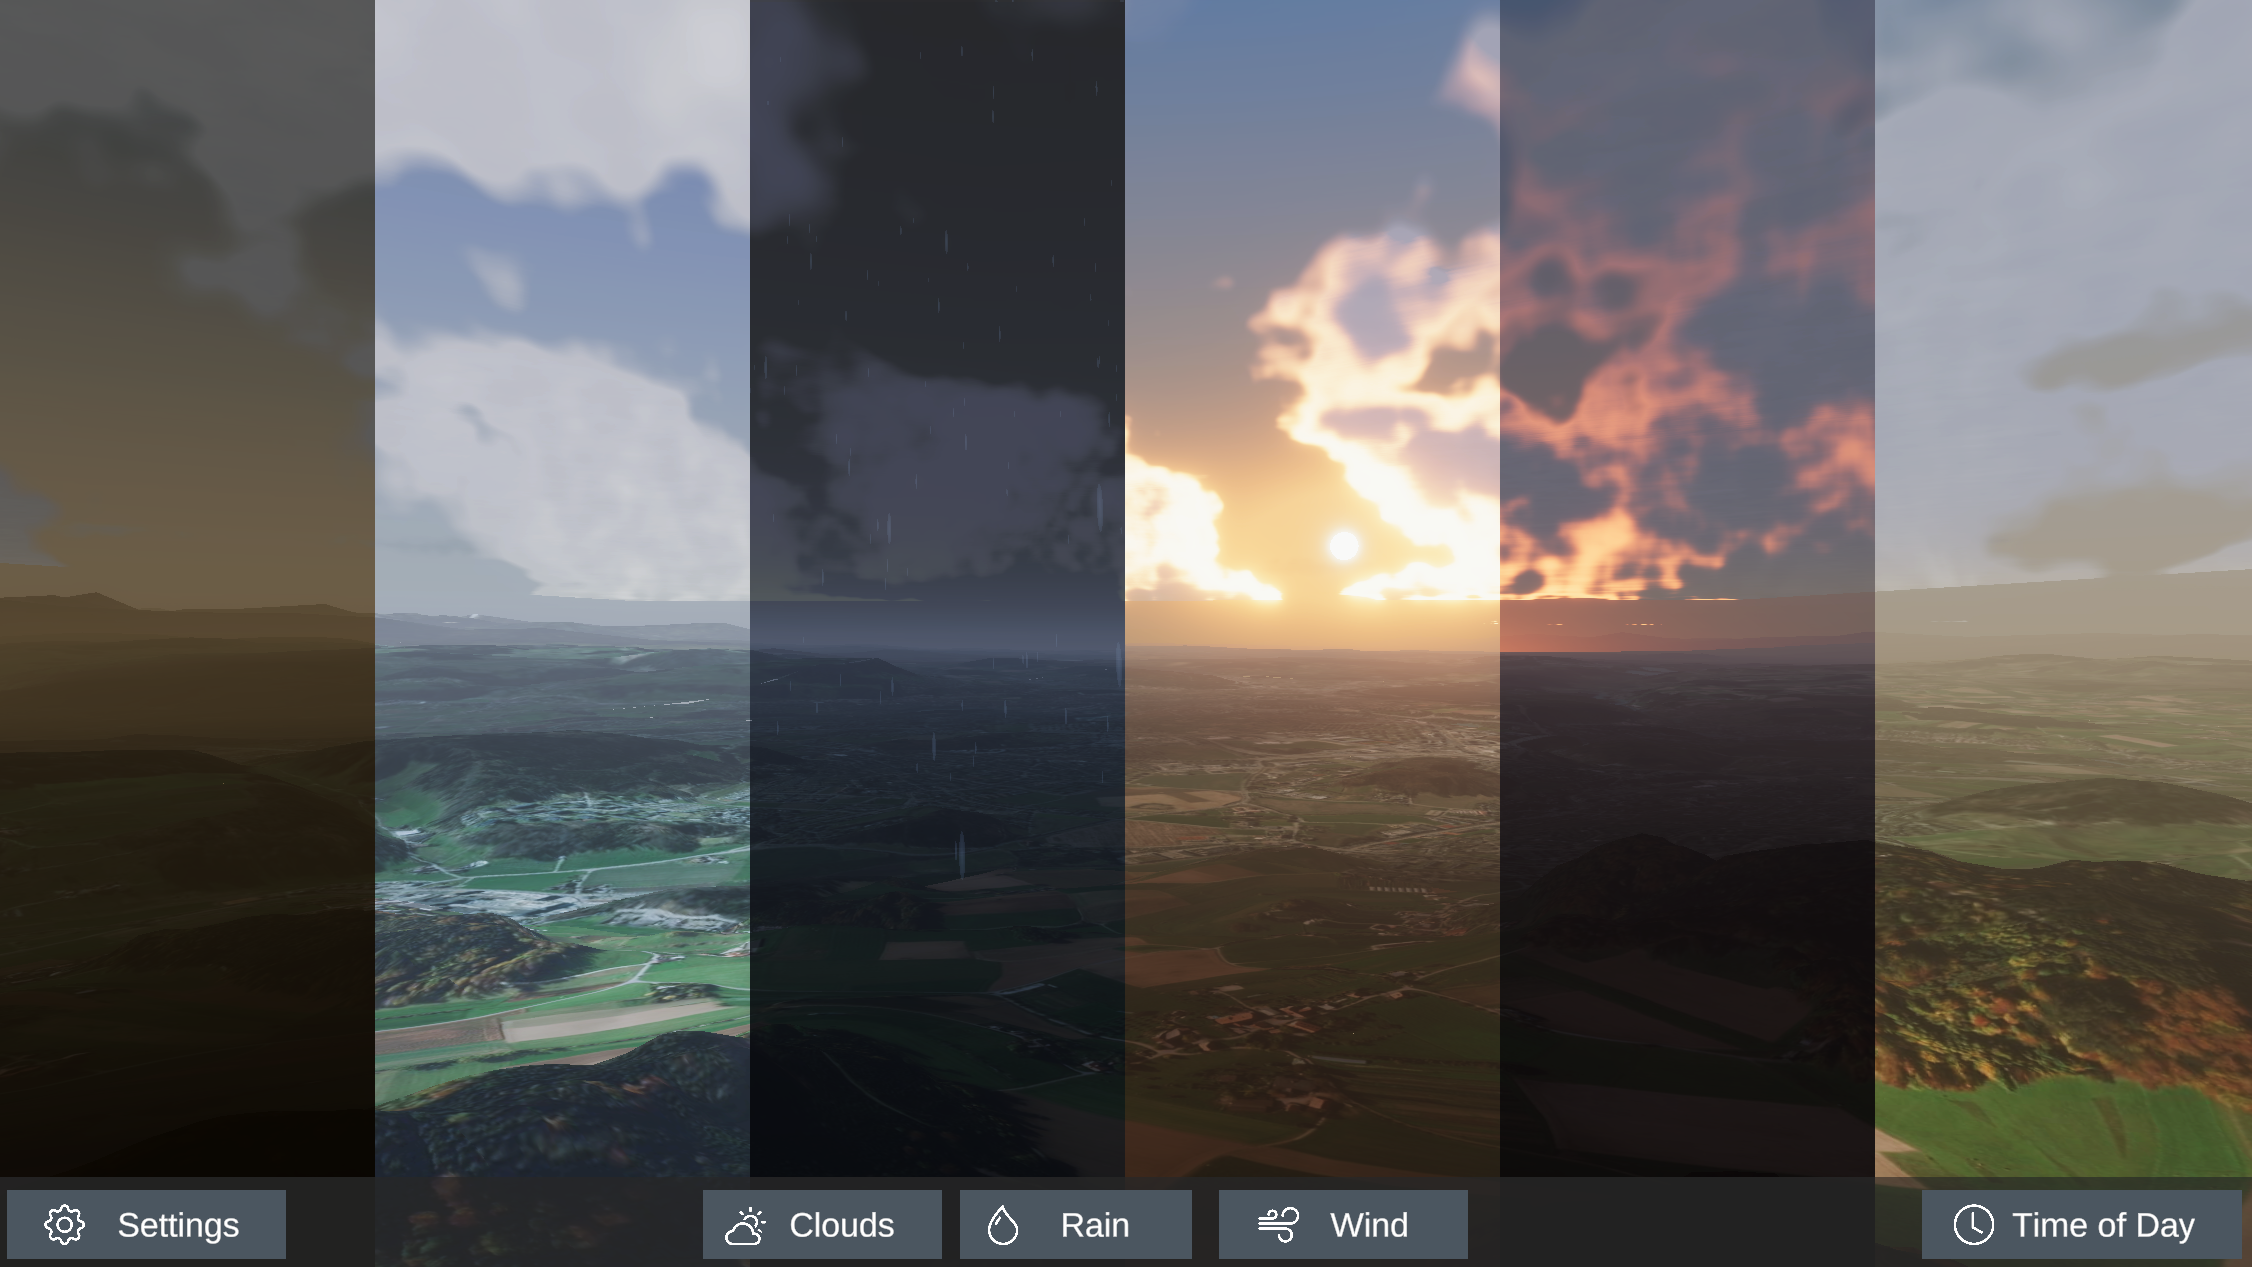
\includegraphics[width=\linewidth]{results/wheel.png}
\end{figure}

\fontsize{10pt}{12pt}\selectfont
\begin{textblock}{150}(28,225)
\begin{tabbing}
xxxxxxxxxxxxxxxxxxxxx\=xxxxxxxxxxxxxxxxxxxxxxxxxxxxxxxxxxxxxxxxxxxxxxx \kill
Field of Studies:	\> \fieldofstudies	\\
Specialization:	    \> \specialisation	\\
Author:		        \> \docauthor \\
Supervisor:         \> \prof \\
Date:			    \> \versiondate \\
Version:		    \> 1.0 \\
\end{tabbing}

\end{textblock}

\begin{textblock}{150}(28,280)
\noindent 
\color{bfhgrey}\fontsize{9pt}{10pt}\selectfont
Berner Fachhochschule | Haute \'ecole sp\'ecialis\'ee bernoise | Bern University of Applied Sciences
\color{black}\selectfont
\end{textblock}

\end{flushleft}

\end{titlepage}
\clearpage

\section*{Abstract}
Clouds contribute a great deal to the overall ambience in games, but an implementation of such effects often proves to be more challenging than anticipated.
To get as close as possible to real clouds, this project engages in researching and developing a near real-time weather rendering system.
This means that real weather forecasts from \emph{meteoblue} are used to visualize past, current and future weather at any given time of day.
The environment is created with elevation model data from \emph{ArcGIS}. Live photographs from \emph{Roundshot} cameras can be viewed side-by-side with the rendered output.
\\
The document dives into the science of clouds and illustrates the ten distinct classifications and how each of those could be represented in a weather simulation. 
In order to achieve high fidelity, the implementation relies on concepts like Voronoi \gls{noisegeneration} and \gls{raymarching}, which means to generate a random 3D cloud pattern and render it in volumetrically.
\\
At last, the goal of the project is to create a fully fledged, near real-time weather rendering system in Unity.
It is able to render \gls{procedural} and volumetric cloudscapes, for any given date and time.
A intuitive user interface allows the user to control the weather simulation manually or let it run automatically based on the \emph{meteoblue} weather reports.
\\
For future work, the weather rendering system could be incorporated in a game or further improved to achieve even higher visual realism.
\clearpage

\tableofcontents
\clearpage

\pagenumbering{arabic}

\section{General}

\subsection{Purpose}
This document serves the purpose of defining and clarifying the goals, which the thesis 'Realtime Weather Rendering System' is supposed to achieve. Furthermore, the requirement specification allows for a more accurate evaluation of the achievement of objectives and of the result itself.

\subsection{Revision History}
\begin{tabularx}{\textwidth}{|l|l|l|X|}
    \hline
    \textbf{Version}         & \textbf{Date}        & \textbf{Name}     & \textbf{Comment}                  \\ \hline \addtocounter{versionnumber}{1}
    0.\arabic{versionnumber} & February 27, 2021    & Matthias Thomann  & Initial draft                     \\ \hline \addtocounter{versionnumber}{1}
    0.\arabic{versionnumber} & March 03, 2021       & Matthias Thomann  & Updated project schedule          \\ \hline
\end{tabularx}
\clearpage
\section{Natural Clouds}
Clouds are a substantial part of Earth's weather. They provide shade from the glistening sun on hot days and reflect the heat at night, keeping the ground warmer.
For a layman, clouds are comprehensible and useful indicators for telling the weather.
If they are dark and low-hanging, they usually bring rain.
If they are puffy and scarce, they predict fair weather ahead.

\subsection{Convection}
\label{section:clouds:convection}
In meteorology, \gls{convection} describes the event of atmospheric motions in the vertical direction.
Hot air rises from Earth's surface in form of bubbles, which are called \emph{\gls{thermal}s}.
As the \gls{altitude} increases, the thermals cool down. At some point, the warm air mixes with the surrounding colder air, after which its moisture condenses and starts forming clouds \cite{weather:convection}.

\begin{figure}[H]
    \centering
    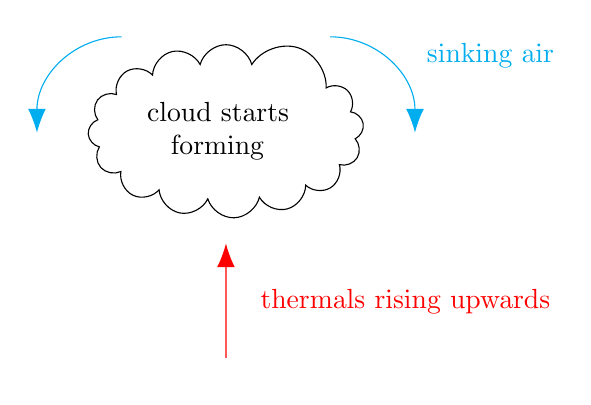
\begin{tikzpicture}[scale=1.2]
        \tikzset{edge/.style = {-{Latex[length=3mm]},shorten >= -4pt}}
        \tikzset{shortedge/.style = {-{Latex[length=3mm]},shorten <=-4pt,shorten >= -4pt}}
        \tikzset{line/.style = {shorten >=-4pt}}
        \tikzset{icon/.style = {font=\Large}}

        % clouds
        \node[text width=2cm] (cloud) at (4.0, 3.0) {cloud starts \phantom{x} forming};
        \node[cloud, rotate=0, cloud puffs=15.7, cloud, minimum width=3.5cm, minimum height=2.2cm, align=center, draw] (cloud) at (cloud) {};

        % thermal
        \node (t1) at (4, 0.5) {};
        \node[red] (t1t) at (5.9, 1.2) {thermals rising upwards};
        \node (t2) at (4, 1.8) {};
        \draw[red,edge] (t1) -- (t2);

        % cold air
        \node (l1) at (3, 4.0) {};
        \node (l2) at (2, 3.0) {};
        \node (r1) at (5, 4.0) {};
        \node (r2) at (6, 3.0) {};
        \node[cyan] (r2t) at (6.8, 3.8) {sinking air};
        \draw[cyan,edge] (l1) to [out=180,in=90] (l2);
        \draw[cyan,edge] (r1) to [out=0,in=90] (r2);

        \end{tikzpicture}
    \captionof{figure}{Lifting by convection.}
    \label{img:tikz:convection}
\end{figure}

\noindent
A \gls{thermal} does not have to rise naturally. It can also be pushed upwards by a cold front.

\begin{figure}[H]
    \centering
    \begin{minipage}{0.47\linewidth}
        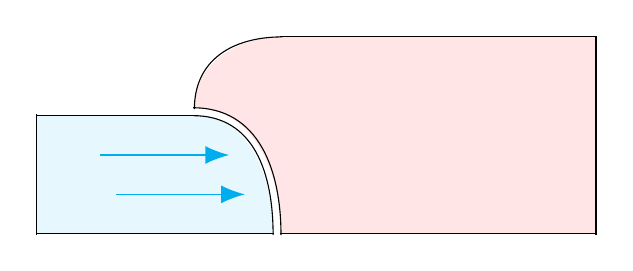
\begin{tikzpicture}
            \tikzset{edge/.style = {-{Latex[length=3mm]},shorten >= -4pt}}
            \tikzset{shortedge/.style = {shorten <=-4pt,shorten >= -4pt}}

            % cold front
            \node (c1) at (0, 0) {};
            \node (c2) at (3, 0) {};
            \node (c3) at (2, 1.5) {};
            \node (c4) at (0, 1.5) {};

            \fill[fill=cyan!10] (0, 0) node {}
                to [] (3,0) node {}
                to [out=90,in=0] (2,1.5) node {}
                to [] (0,1.5) node {};
            \draw[shortedge] (c1) to [] (c2);
            \draw[shortedge] (c2) to [out=90,in=0] (c3);
            \draw[shortedge] (c3) to [] (c4);
            \draw[shortedge] (c4) to [] (c1);
            
            % warm front
            \node (w1) at (3.1, 0) {};
            \node (w2) at (7.1, 0) {};
            \node (w3) at (7.1, 2.5) {};
            \node (w4) at (3.1, 2.5) {};
            \node (w5) at (2, 1.6) {};

            \fill[fill=red!10] (7.1, 0) node {}
                to [] (7.1,2.5) node {}
                to [] (3.1,2.5) node {}
                to [out=180,in=90] (2,1.6) node {}
                to [out=0,in=90] (3.1,0) node {};
            \draw[shortedge] (w1) to [] (w2);
            \draw[shortedge] (w2) to [] (w3);
            \draw[shortedge] (w3) to [] (w4);
            \draw[shortedge] (w4) to [out=180,in=90] (w5);
            \draw[shortedge] (w5) to [out=0,in=90] (w1);

            % cold front arrows
            \draw[cyan,edge] (1,0.5) -- (2.5,0.5);
            \draw[cyan,edge] (0.8,1) -- (2.3,1);
        \end{tikzpicture}
        \captionof{figure}{Convection: Cold front approaching.}
        \label{img:tikz:convection:cold1}
    \end{minipage}        
    \hfill
    \begin{minipage}{0.47\linewidth}
        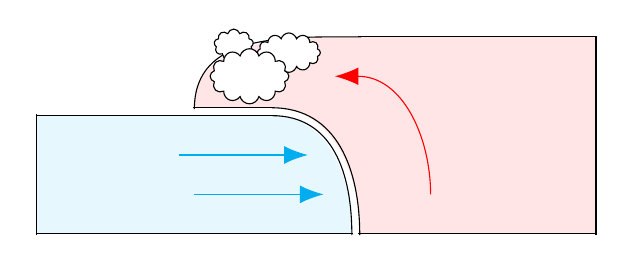
\begin{tikzpicture}
            \tikzset{edge/.style = {-{Latex[length=3mm]},shorten >= -4pt}}
            \tikzset{shortedge/.style = {shorten <=-4pt,shorten >= -4pt}}

            % cold front
            \node (c1) at (0, 0) {};
            \node (c2) at (4, 0) {};
            \node (c3) at (3, 1.5) {};
            \node (c4) at (0, 1.5) {};

            \fill[fill=cyan!10] (0, 0) node {}
                to [] (4,0) node {}
                to [out=90,in=0] (3,1.5) node {}
                to [] (0,1.5) node {};
            \draw[shortedge] (c1) to [] (c2);
            \draw[shortedge] (c2) to [out=90,in=0] (c3);
            \draw[shortedge] (c3) to [] (c4);
            \draw[shortedge] (c4) to [] (c1);
            
            % warm front
            \node (w1) at (4.1, 0) {};
            \node (w2) at (7.1, 0) {};
            \node (w3) at (7.1, 2.5) {};
            \node (w4) at (4.1, 2.5) {};
            \node (w5) at (2, 1.6) {};
            \node (w6) at (3, 1.6) {};

            \fill[fill=red!10] (7.1, 0) node {}
                to [] (7.1,2.5) node {}
                to [] (4.1,2.5) node {}
                to [out=180,in=90] (2,1.6) node {}
                to [] (3,1.6) node {}
                to [out=0,in=90] (4.1,0) node {};
            \draw[shortedge] (w1) to [] (w2);
            \draw[shortedge] (w2) to [] (w3);
            \draw[shortedge] (w3) to [] (w4);
            \draw[shortedge] (w4) to [out=180,in=90] (w5);
            \draw[shortedge] (w5) to [] (w6);
            \draw[shortedge] (w6) to [out=0,in=90] (w1);

            % cold front arrows
            \draw[cyan,edge] (2,0.5) -- (3.5,0.5);
            \draw[cyan,edge] (1.8,1) -- (3.3,1);
            
            % warm front arrows
            \node (wf) at (3.8,2) {};
            \draw[red,edge] (5,0.5) to [out=90,in=0] (wf);

            % clouds
            \node (cloud1) at (2.5, 2.4) {};
            \node (cloud2) at (3.2, 2.3) {};
            \node (cloud3) at (2.7, 2) {};
            \node[cloud,fill=white,cloud puffs=9, cloud, minimum width=0.5cm, minimum height=0.2cm, align=center, draw] (cloud) at (cloud1) {};
            \node[cloud,fill=white,cloud puffs=12, cloud, minimum width=0.8cm, minimum height=0.5cm, align=center, draw] (cloud) at (cloud2) {};
            \node[cloud,fill=white,cloud puffs=12, cloud, minimum width=1.0cm, minimum height=0.7cm, align=center, draw] (cloud) at (cloud3) {};

        \end{tikzpicture}
        \captionof{figure}{Convection: Cold front pushing creating thermals.}
        \label{img:tikz:convection:cold2}       
    \end{minipage}
\end{figure}

\subsection{Weather Fronts}
According to \emph{metoffice} \cite{metoffice:weatherfronts}, weather fronts are boundaries between two air masses. Those masses differ in temparature and humidity.
There are three types of weather fronts: \emph{cold}, \emph{warm} and \emph{occluded} fronts.

\subsubsection{Cold Front}
A cold front speaks of cool air that is moved forwards. As colder air is denser than warmer air, it pushes underneath the warmer air.
By pushing up warm air, \gls{thermal}s are created and clouds start to form.

\subsubsection{Warm Front}
Different to the cold front, a warm front carries warmer air and therefore rises over the colder, denser air.
Still, by advancing above the cold air, the warm front pushes the warmer air higher, which means that in this case too, \gls{thermal}s are created and clouds start to form.

\subsubsection{Occluded Front}
\color{orange}
TODO
\color{black}

\subsection{Classifications}
In order to create a \gls{wrs} that is able to display many different cloudscapes, all types of clouds have to be understood first.
The \gls{wmo} describes ten distinct cloud classifications. For each of those, there are further subtypes. For simplicity, those subtypes will be disregarded in this project.

\begin{figure}[H]
    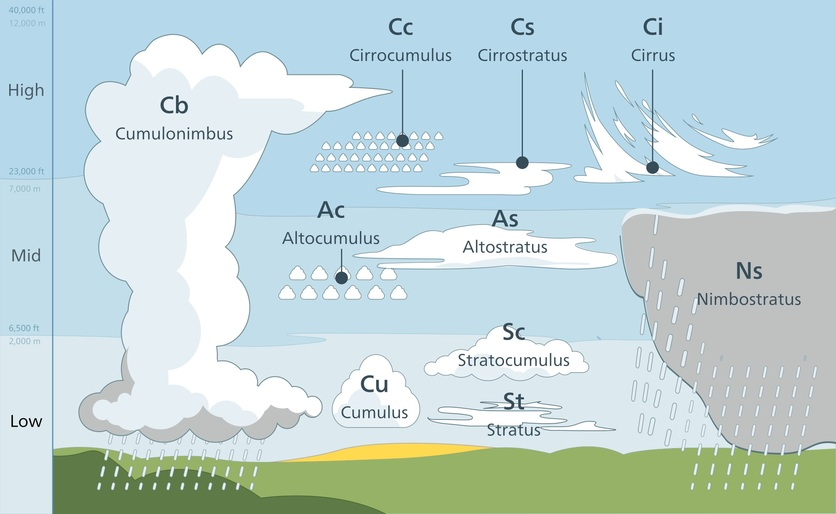
\includegraphics[width=\linewidth]{clouds-types.jpg}
    \captionof{figure}{Distinct classifications of cloudshapes in the troposphere \protect\cite{cloudtypes:wiki}.}
    \label{img:ui:mockup:live}
\end{figure}

\noindent
This graphic above provides and excellent overview of all distinct cloud types.
Each type is depicted in its signature shape and marked with the scientific name and abbreviation.
Natural clouds are typically identified by two major factors: shape and \gls{altitude}.
The \gls{altitude}, which is the distance from sea level to the cloud, is further split into three categories "low", "mid" and "high".
This corresponds to the altitude at which the cloud usually forms, up to twelve kilometers above ground. 
\\
All of those clouds are formed in the troposphere, Earth's lowest atmospheric layer.
Certain clouds may occur in the stratospheric or even the mesospheric layer, but they are usually a rare sight. Therefore, those clouds will not be covered in this project.

% refs:
% https://www.countryfile.com/how-to/outdoor-skills/how-to-predict-the-weather-forecast-using-clouds/
% NASA how do clouds form: https://climatekids.nasa.gov/cloud-formation/#:~:text=Clouds%20are%20created%20when%20water,are%20floating%20in%20the%20air.&text=That%20means%20some%20of%20the,drifted%20away%20into%20the%20atmosphere.
% NASA: https://www.nasa.gov/audience/forstudents/k-4/stories/nasa-knows/what-are-clouds-k4.html
% http://ww2010.atmos.uiuc.edu/(Gh)/wwhlpr/cold_front_precip.rxml?hret=/guides/mtr/cld/cldtyp/mdl/altcu.rxml
% https://content.meteoblue.com/en/meteoscool/weather/clouds/cloud-types

\pagebreak

\subsubsection{Cirrus}
\begin{wrapfigure}[10]{r}{6cm}
    \vspace{-\baselineskip}
    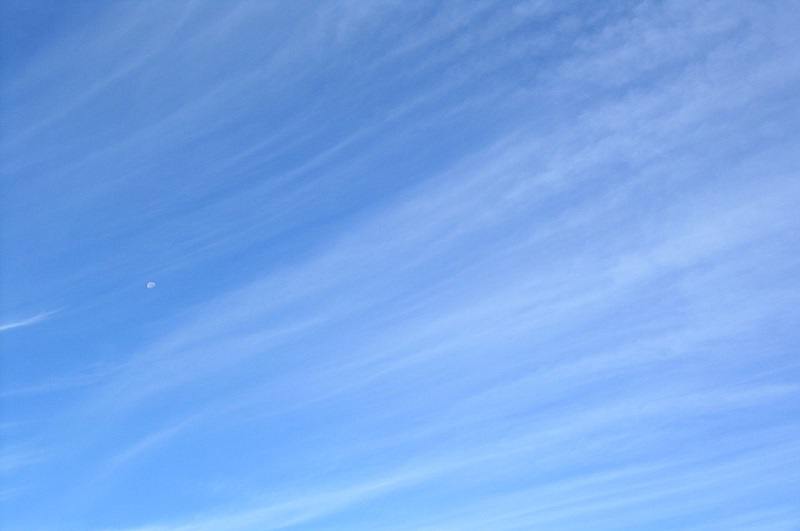
\includegraphics[width=6cm]{clouds/cirrus.jpg}
    \caption{Cirrus clouds \protect\cite{cloudtypes:wiki:cirrus}.}
    \label{img:clouds:cirrus}
\end{wrapfigure}
Cirrus clouds consist of thin, hair-like strands.
They fall into the "high" altitude group and mostly appear in a bright white color, although they may take on the colors of the sunset or sunrise.
Typically, they are formed when \gls{watervapor} undergoes \gls{desublimation}, the process in which gas turns into solid. This occurs when the \gls{watervapor} freezes rapidly at high altitudes, turning into ice crystals.
\\
\noindent
However, cirrus clouds can also form from air that flows outwards of thunderstorms.
\emptyline
\textbf{Interpretation:} Fair weather, but they might announce the arrival of warm front in 12-24 hours, which is often preceded by rain several hours in advance.
Even though cirrus clouds indicate \gls{precipitation}, they themselves do not produce rainfall \cite{predict:weather}.

\subsubsection{Cirrostratus}
\begin{wrapfigure}[10]{r}{6cm}
    \vspace{-\baselineskip}
    
\includegraphics[width=6cm]{clouds/cirrostratus.jpg}
    \caption{Cirrostratus clouds \protect\cite{cloudtypes:wiki:cirrostratus}.}
    \label{img:clouds:cirrostratus}
\end{wrapfigure}
Cirrostratus clouds are similar to the cirrus clouds, only that they are even thinner.
Those clouds depict more of a veil than a single cloud shape.
They form under the same conditions as the cirrus clouds and can cover a massive area of the sky, spanning thousands of kilometers.
\\
\noindent
Cirrostratus clouds sometimes produce white rings or arcs of lights around the sun or the moon called the \emph{\gls{halophenomenon}}.
Sometimes, the cirrostratus clouds are so thin that the halo is the only way to tell if there are cirrostratus clouds.
\emptyline
\textbf{Interpretation:} Fair weather, but they indicate a warm front within one or two days, bringing \gls{precipitation} \cite{cloudtypes:meteoblue}.

\subsubsection{Cirrocumulus}
\begin{wrapfigure}[10]{r}{6cm}
    \vspace{-\baselineskip}
    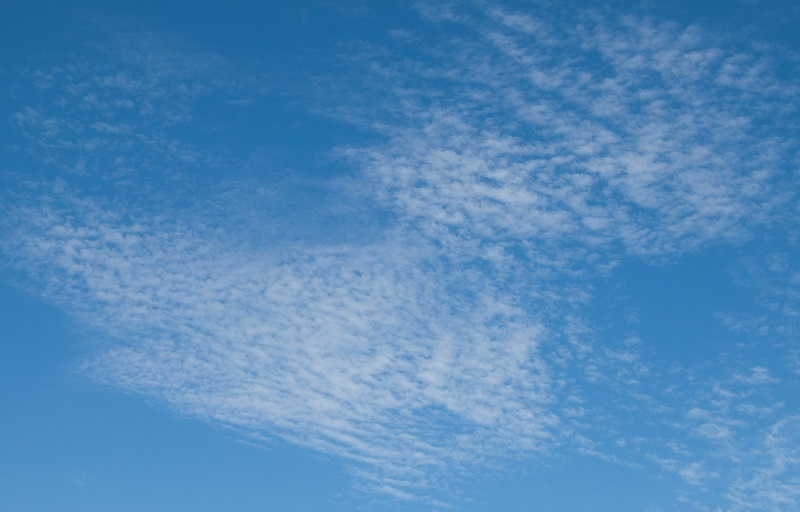
\includegraphics[width=6cm]{clouds/cirrocumulus.jpg}
    \caption{Cirrocumulus clouds \protect\cite{cloudtypes:wiki:cirrocumulus}.}
    \label{img:clouds:cirrocumulus}
\end{wrapfigure}
Similar to the other clouds of the cirrus-family, the cirrocumulus are composed of ice crystals and formed at high \gls{altitude}s.
They are made up of many small, white, puffy clouds called \emph{\gls{cloudlet}}s. Their wooly look give the cloud the name \emph{cumulus}.
\\
\noindent
Cirrocumulus clouds are realtively rare, as they are naturally only formed when a turbulent vertical current meets a cirrus cloud layer. The cirrus cloud then disperses into many \gls{cloudlet}s.
\emptyline
\textbf{Interpretation:} 
They do produce \gls{precipitation}, but it never reaches the surface, meaning that cirrocumulus clouds are typically associated with fair weather \cite{cloudtypes:meteoblue}.

\clearpage

\subsubsection{Altostratus}
\begin{wrapfigure}[10]{r}{6cm}
    \vspace{-\baselineskip}
    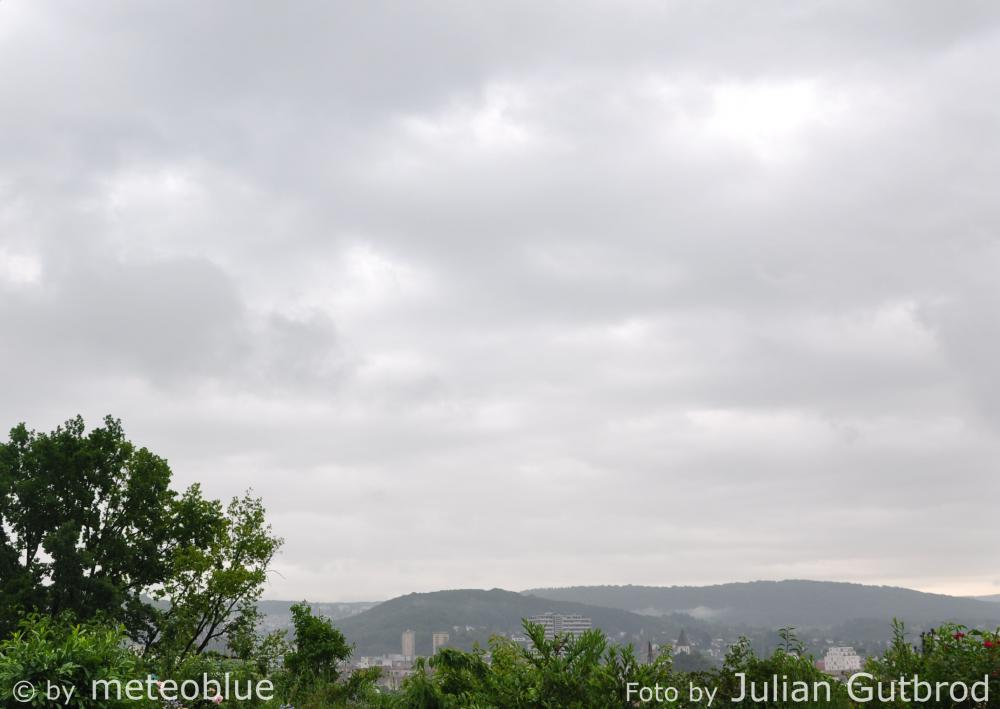
\includegraphics[width=6cm]{clouds/altostratus.jpg}
    \caption{Altostratus clouds \protect\cite{cloudtypes:meteoblue}.}
    \label{img:clouds:altostratus}
\end{wrapfigure}
The name for this grey, uniform sheet of clouds consists of the latin words \emph{alto} (height) and \emph{stratus} (layered), summing up their appearance accurately.
Altostratus clouds usually cover the whole sky and form a dull blanket of monocolored clouds with very few features.
The sun- or moonlight may shine through them, but will most likely not be strong enough to cast defined shadows.
\emptyline
\textbf{Interpretation:}
Altostratus clouds usually indicate \gls{precipitation}, even more so if they are are preceded by cirrus clouds.
If the \gls{precipitation} increases in persistence and intensity, the altostratus clouds will lower and thicken into nimbostratus clouds.


\subsubsection{Altocumulus}
\begin{wrapfigure}[9]{r}{6cm}
    \vspace{-\baselineskip}
    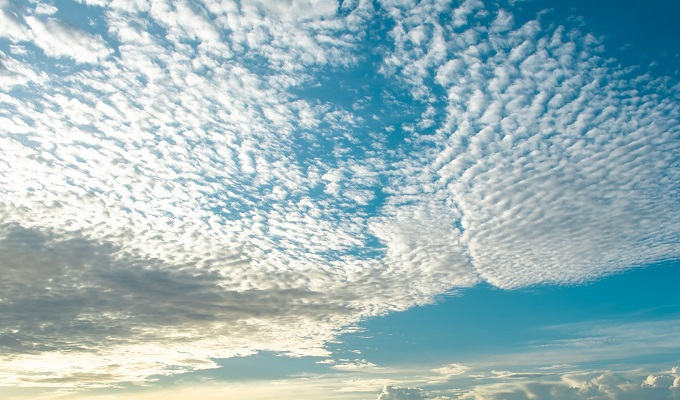
\includegraphics[width=6cm]{clouds/altocumulus.jpg}
    \caption{Altocumulus clouds \protect\cite{cloudtypes:wiki:altocumulus}.}
    \label{img:clouds:altocumulus}
\end{wrapfigure}
As with the cirrocumulus clouds, altocumulus clouds consist of small, puffy, white and grey \gls{cloudlet}s.
These \gls{cloudlet}s are usually slightly bigger than the ones of the cirrocumulus cloud.
It is easy to tell them apart, as the altocumulus \gls{cloudlet}s are usually more grey than white and are shaded on one side.
Altocumulus clouds can form through the dispersion of altostratus clouds or through \gls{convection} (see \sectionref{section:clouds:convection}).
\emptyline
\textbf{Interpretation:}
Usually, they are found in settled weather. They do not produce \gls{precipitation} that reaches the surface.


\subsubsection{Nimbostratus}
\begin{wrapfigure}[10]{r}{6cm}
    \vspace{-\baselineskip}
    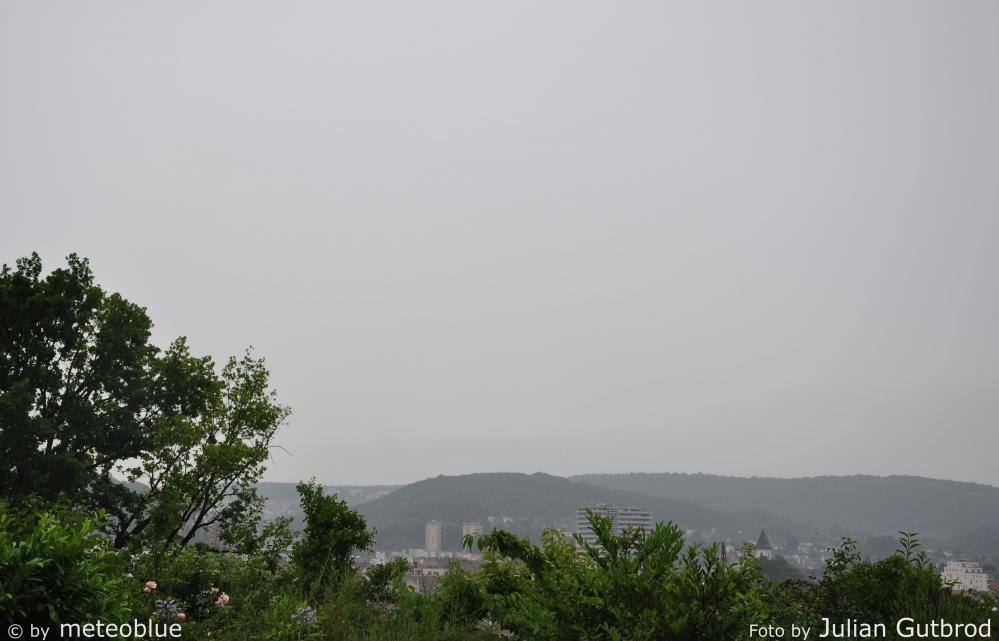
\includegraphics[width=6cm]{clouds/nimbostratus.jpg}
    \caption{Nimbostratus clouds \protect\cite{cloudtypes:wiki:nimbostratus}.}
    \label{img:clouds:nimbostratus}
\end{wrapfigure}
The nimbostratus clouds are the vast, grey clouds that bring heavy rain or snow for a longer period of time, sometimes up to multiple days.
With their dark and gloomy appearance, they convey a dreary mood along with the persistent \gls{precipitation}.
\\
The thick, featureless layers of cloud are often formed by \gls{occludedfront}s, when an altostratus starts lowering and gets denser.
\emptyline
\textbf{Interpretation:}
They bring long-term rain or snow for several hours or days.
\clearpage

\printnoidxglossary 
\clearpage
\printbibliography[heading=bibintoc]
\clearpage
\phantomsection
\addcontentsline{toc}{section}{Listings}
\phantomsection
\addcontentsline{toc}{subsection}{Figures}
\listoffigures
\clearpage
\phantomsection
\addcontentsline{toc}{subsection}{Code Listings}
\lstlistoflistings

\end{document}
